\chapter{Macchina aritmetica}

\section{Macchina aritmetica}

Progettare e implementare in VHDL una macchina aritmetica sequenziale a scelta fra le seguenti: 
    \begin{itemize}
        \item moltiplicatore di Robertson, per effettuare il prodotto di 2 stringhe A e B da 8 bit ciascuna;
        \item moltiplicatore di Booth, per effettuare il prodotto di 2 stringhe A e B da 8 bit ciascuna;
        \item divisore non-restoring, per effettuare la divisione intera fra due stringhe A e B di 4 bit ciascuna;
        \item divisore restoring, per effettuare la divisione intera fra due stringhe A e B di 4 bit ciascuna;
    \end{itemize}

Opzionalmente, la macchina implementata può essere sintetizzata su FPGA e testata mediante l’utilizzo dei dispositivi di input/output (switch, bottoni, led, display) presenti sulla board di sviluppo in dotazione al gruppo. La modalità di utilizzo degli stessi è a completa discrezione degli studenti.


\subsection{Il moltiplicatore di Robertson}
Si è scelto di implementare il moltiplicatore di Robertson. Nella prima sezione sarà descritta la parte architetturale con alcuni riferimenti teorici, mentre in quella successiva si scenderà nei dettagli implementativi e nel codice, esaminando il funzionamento della macchina attraverso i \textit{testbench}.

\subsubsection{Architettura}
L'architettura del sistema può essere suddivisa in due parti: l'unità di controllo e l'unità operativa.
Il sistema prende in ingresso i due operandi a 8 bit, i segnali di start, clock e reset e presenta in uscita il risultato della moltiplicazione a 16 bit, oltre che a due segnali di stop, che indicano la fine dell'operazione.
Dal seguente schema è possibile identificare i diversi componenti. Tutti i componenti diversi dalla UC (Unità di Controllo) costituiscono la parte operativa.
L'algoritmo manuale della moltiplicazione su N bit può essere formalizzato nella seguente espressione:
\begin{equation*}
  \mathlarger{\sum}_{i=0}^{N-1}X_i\cdot2^i\cdot Y
      \label{eq:mul_alg}
\end{equation*}


\begin{figure}[H]
    \centering
    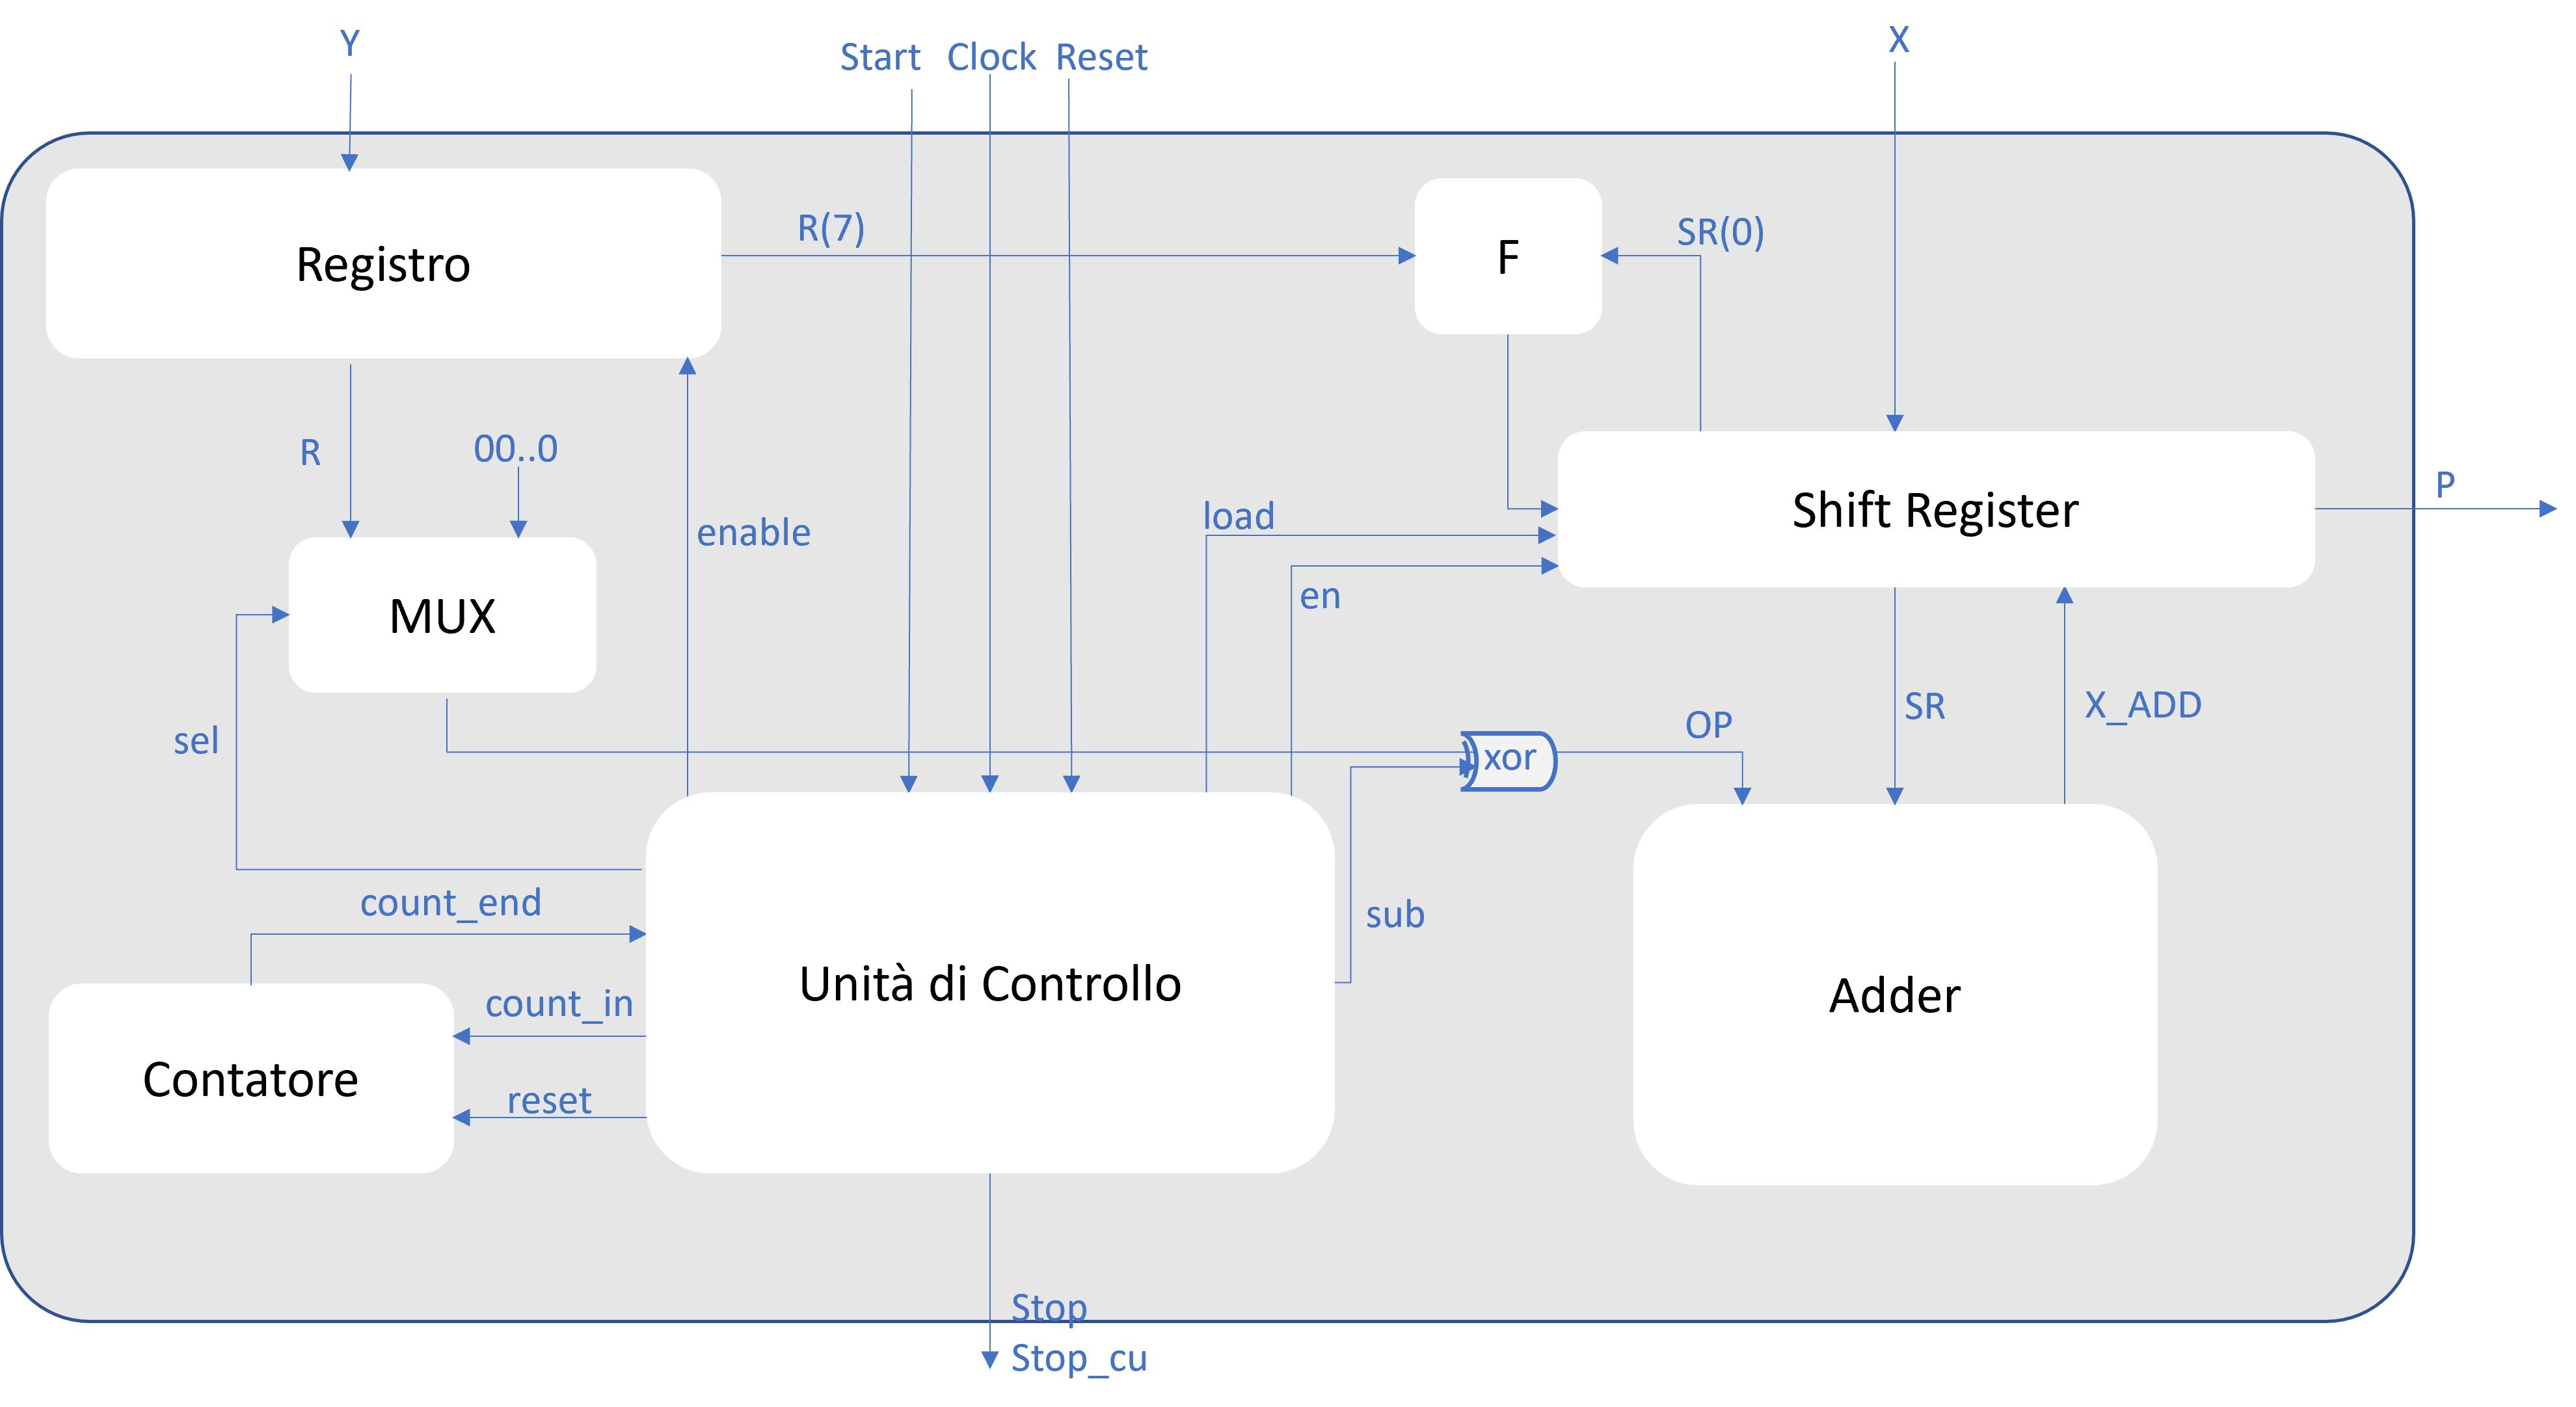
\includegraphics[width=17cm]{immagini/esercizio11/robertson_arch.png}
    \caption{Architettura moltiplicatore di Robertson}
    \label{fig:robertson_arch}
\end{figure}

L'unità operativa è formata dai seguenti componenti:
\begin{itemize}
\item \textbf{Shift register}: un registro a scorrimento a 16 bit in cui negli 8 meno significativi viene memorizzato l'operando X. L'unità di controllo decide se caricare l'operando o i risultati parziali del sommatore attraverso i segnali \textit{load} e \textit{load\_add}, e a ogni colpo di clock viene effettuato uno shift verso destra. Il motivo per cui si esegue lo \textit{shift} verso destra ha a che fare con l'algoritmo su cui si basa il moltiplicatore: partendo dall'algoritmo della moltiplicazione manuale, bisognerebbe variare il numero di \textit{shift} a sinistra in base al passo corrente durante (dalla Equazione \ref{eq:mul_alg} si vede che lo \textit{shift} dipende dalla $i$) il calcolo delle somme parziali. Per evitare questo problema si esegue prima la somma parziale e poi si scorre ogni volta verso destra di una sola posizione.

\item \textbf{Registro}:  un registro a 8 bit che memorizza il valore dell'operando Y. Oltre all'uscita a 8 bit che entra nel \textit{multiplexer}, contenente l'operando stesso, viene fornito il bit più significativo a F per il calcolo del segno.
\item \textbf{Contatore}: serve a contare i passi dell'unità di controllo. Quando arriva al massimo valore viene alzato il segnale \textit{cont\_end} e viene effettuata l'eventuale correzione che dipende dai segni degli operandi (come illustrato nella sezione dell'unità di controllo)
\item \textbf{Adder}: un \textit{ripple carry adder} che esegue le somme parziali e che è in grado anche di eseguire le sottrazioni. Per effettuare questo cambio, da somma a sottrazione, si usa un segnale di controllo sub che entra insieme all'uscita del \textit{multiplexer} (che conterrà Y) in una XOR, che a sua volta è collegata all'adder. In questo modo può essere calcolato -B in complementi a due. Per la somma normale l'entrata della XOR rappresenta invece il riporto entrante.
\item \textbf{F}: un registro che contiene il bit relativo al segno che viene calcolato come (Y(7) and X(0))or F).
\end{itemize}

L'unità di controllo è realizzata mediante un automa a stati finiti, il cui schema è mostrato in figura:

\begin{figure}[H]
    \centering
    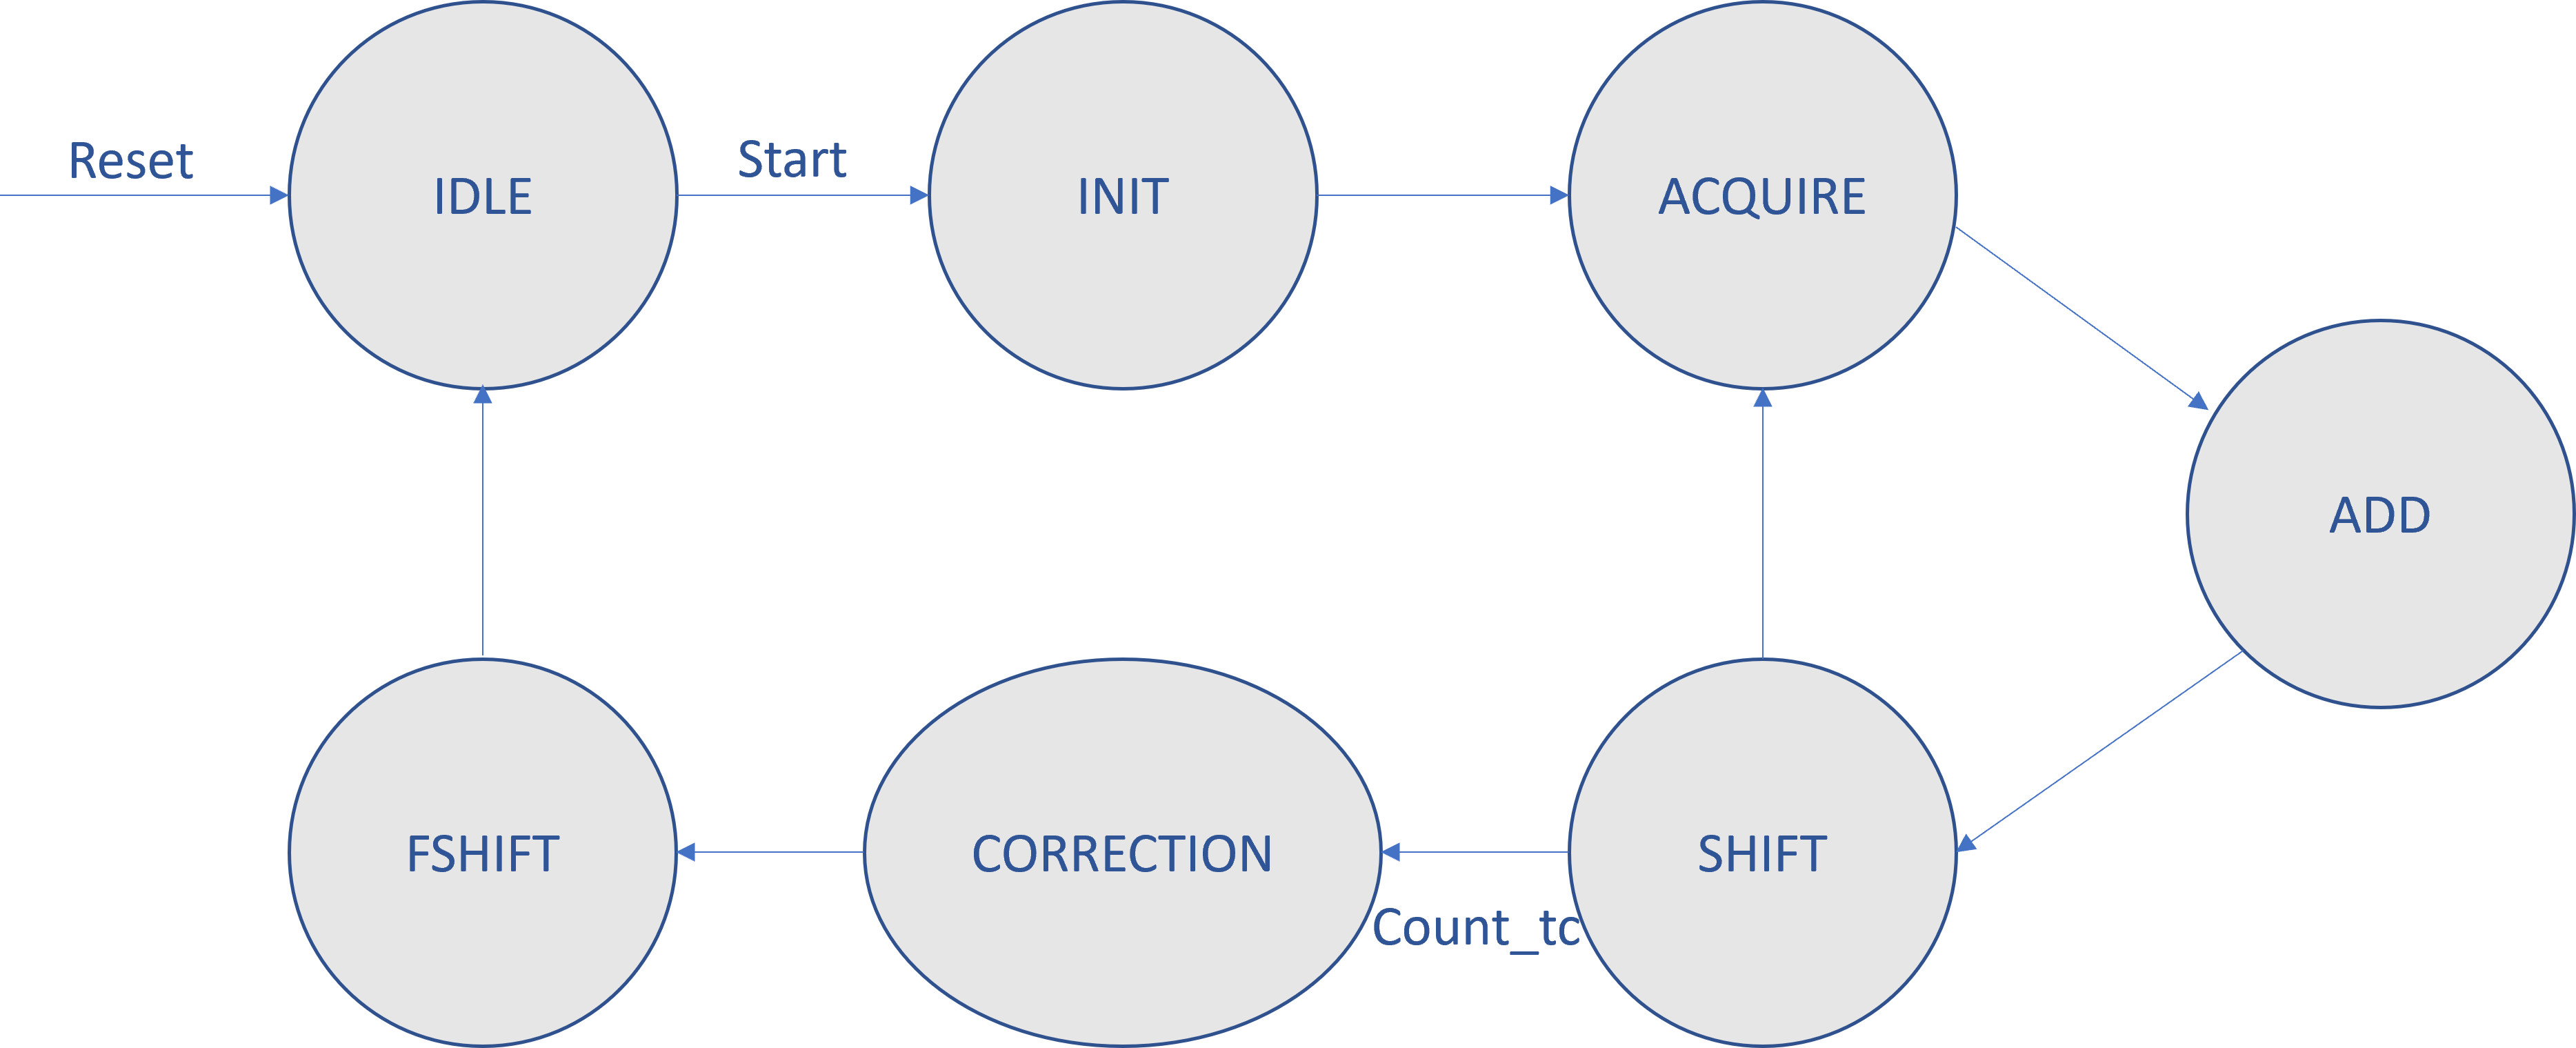
\includegraphics[width=14cm]{immagini/esercizio11/automa_robertson.png}
    \caption{Automa Moltiplicatore Robertson}
    \label{fig:robertson_automa}
\end{figure}

Di particolare importanza è il penultimo stato di correzione, necessario quando il risultato è negativo. Mentre il valore di Y è noto fin da subito, quindi non pone problemi anche nel caso sia negativo, X è conosciuto solo negli ultimi stati, dove a quel punto si è arrivati facendo la somma normale. Per far si che il risultato sia corretto vengono gestiti quindi i diversi casi:
\begin{itemize}
\item $X, Y >0$: non sono necessarie correzioni;
\item $X>0, Y<0$: grazie a F viene conservato il segno del prodotto negativo con Y, quindi non sono necessarie correzioni;
\item $X<0, Y>0$: è necessario il passo di correzione in cui si effettua la sottrazione al posto della somma;
\item $X, Y <0$: è necessario il passo di correzione per rendere il risultato positivo.
\end{itemize}


Nel listato \ref{robertson_op} è riportato il codice dell'unità operativa del molitplicatore di Robertson. Come descritto nell'architettura instanzia l'addizionatore (che può diventare un sottrattore a richiesta, invertendo il secondo operandoO), un registro a scorrimento (in cui sono memorizzati sia l'operando iniziale che il risultato finale) e un registro per il secondo operando e un contatore per tenere traccia dello stato delle operazioni.


\begin{lstlisting} [language=VHDL, label=robertson_op, caption=Unità operativa]
library IEEE;
use IEEE.STD_LOGIC_1164.ALL;
use IEEE.NUMERIC_STD.ALL;

entity unita_operativa is
	port( X, Y: in std_logic_vector(7 downto 0);
		  clock, reset, load, sub, sel: in std_logic;
		  en_SR, en_R8, en_D, count_in, load_add, shift, f_shift: in std_logic;
		  count: out std_logic_vector(2 downto 0);
		  P: out std_logic_vector(15 downto 0));
end unita_operativa;

architecture structural of unita_operativa is

	component adder_sub is
	port( X, Y: in std_logic_vector(7 downto 0);
		  cin: in std_logic;
		  Z: out std_logic_vector(7 downto 0);
		  cout: out std_logic);		  
	end component;
	
	component registro8 is 
	port( A: in std_logic_vector(7 downto 0);
		  clk, res,en: in std_logic;
		  B: out std_logic_vector(7 downto 0));
	end component;
	
	
	component mux_21 is
	port( x0, x1: in std_logic_vector(7 downto 0);
		  s: in std_logic;
		  y: out std_logic_vector(7 downto 0));
	end component;
	
	
	component shif_register is
	port( X: in std_logic_vector(15 downto 0);
		  F: in std_logic;
		  clock, reset, load, en, load_add, shift, f_shift:in std_logic;
		  x_add: in std_logic_vector(7 downto 0);
		  Y: out std_logic_vector(15 downto 0));	  
	end component;
	
	component FFD is
	port( clock, reset, d, en: in std_logic;
          y: out std_logic);
	end component;
	
	component cont_mod8 is
	port( clock, reset: in std_logic;
		  count_in: in std_logic;
		  count_end: out std_logic;
		  count: out std_logic_vector(2 downto 0));
	end component;


	signal temp1: std_logic_vector(7 downto 0);
	signal op1: std_logic_vector(7 downto 0);
	signal temp2: std_logic_vector(15 downto 0); 
	signal temp_p: std_logic_vector(15 downto 0);
	signal temp_d: std_logic :='0';
	signal temp_F: std_logic;
	signal tempadd: std_logic_vector(7 downto 0);
	signal riporto: std_logic;
	signal temp_countend: std_logic;
begin
	M: registro8 port map(Y, clock, reset, en_R8,temp1);
	MUX: mux_21 port map("00000000", temp1, sel, op1);
	
    temp2<="00000000" & X;
	SR: shif_register port map(temp2, temp_F, clock, reset, load, en_SR, load_add, shift, f_shift, tempadd, temp_p);
	temp_d<=(temp1(7) and temp_p(0)) or temp_F;
	D: FFD port map(clock, reset, temp_d, en_D, temp_F);
	ADD_SUB: adder_sub port map(temp_p(15 downto 8), op1, sub, tempadd, riporto);
	CONT: cont_mod8 port map(clock, reset, count_in, temp_countend, count);
	P<=temp_p;

end structural;
\end{lstlisting}

L'unità di controllo si occupa di implementare l'automa mostrato in Figura \ref{fig:robertson_automa}. Nel listato che segue è riportata l'implementazione.
\begin{lstlisting} [language=VHDL, label=robertson_rc, caption=Unità di Controllo]
library IEEE;
use IEEE.STD_LOGIC_1164.ALL;
use IEEE.NUMERIC_STD.ALL;

entity unita_controllo is 
	port( q0, clock, reset, start: in std_logic;
			count: in std_logic_vector(2 downto 0);
		  en_SR, en_R8, en_D, count_in, load_add, en_shift: out std_logic;
		  sel, reset_out, subtract, load, stop, en_fshift, stop_cu: out std_logic); 
end unita_controllo;

architecture Behavioral of unita_controllo is
	type state is (idle, init, acquisizione, add, shift, correzione, f_shift);
	signal current_state, next_state: state;

	begin 

	reg_stato: process(clock, reset)
			  begin
		      if(reset='1') then 
				current_state<=init;
			  elsif(clock'event and clock='1') then 
				current_state<=next_state;
			  end if;
			  end process;
			  
	comb: process(current_state, count)
		  begin
		  next_state<=idle;
		 
		  CASE current_state is
		  
		  WHEN idle => reset_out<='1';
					   en_D<='1';
					   en_R8<='1';
					   en_SR<='1';
					   count_in<='0'; 
					   subtract<='0';
					   load_add<='0';
					   load<='0';
					   sel<='0';
					   stop<='0';
						stop_cu<='0';
						en_fshift<='0';
						en_shift<='0';
					   if(start='1') then next_state<=init;
					   else next_state<=idle;
					   end if;
		--in ogni stato dobbiamo predisporre i valori dei segnali per lo stadio successivo
		  WHEN init => reset_out<='0'; 
		               count_in<='0';
					   load_add<='0';
					   en_D<='1';
					   en_R8<='1';
					   en_SR<='1';
					   load<='1';
					   subtract<='0';
					   stop<='0';
					   sel<=q0;
						en_shift<='0';
						en_fshift<='0';
						stop_cu<='0';
					   next_state<=acquisizione;
						
		--acquisisce gli operandi e predispone la add
		 WHEN acquisizione =>   en_SR<='1';
					  load<='0'; 
					  reset_out<='0'; 
					  en_D<='1';
					  load_add<='1';
					  en_R8<='1';
					  count_in<='1';
					  subtract<='0';
					  sel<=q0;
					  stop<='0';
					  stop_cu<='0';
					  en_fshift<='0';
					  en_shift<='0';
					  if(count="111") then 
									subtract<='1';
									next_state<=correzione;
									
					  else next_state<=add;
					  end if;
		--esegue la somma e predispone lo shift  
		 WHEN add =>  count_in<='0';
					  reset_out<='0'; 
		              sel<=q0;
					  subtract<='0';
					  load_add<='0'; 
					  en_SR<='1'; 
					  en_shift<='1';
					  load<='0'; 
					  en_D<='0';
					  en_R8<='1';
					  stop_cu<='0';
					  stop<='0';
					  en_fshift<='0';
					  next_state<=shift;
		--esegue lo shift e predispone per acquisizione	  
		WHEN shift => load<='0';
					  load_add<='0';
					  en_SR<='1'; --sr abilitato senza caricare x
					  reset_out<='0'; 
		           sel<=q0;
					  en_shift<='0';
					  count_in<='0';
					  subtract<='0';
					  en_D<='0';
					  en_R8<='1';
					  stop_cu<='0';
					  en_fshift<='0';
					  stop<='0';
					  next_state<=acquisizione;
	
	--in correzione fa la sottrazione e predispone per l'ultimo shift
		WHEN correzione => 	en_SR<='1';
							subtract<='0';
							load<='0'; 
							reset_out<='0'; 
							load_add<='0';
							en_D<='0'; --a(7)=a(7)
							en_R8<='1';
							count_in<='0';
							en_shift<='0';
							en_fshift<='1';
							sel<=q0;
							stop<='1';
							stop_cu<='0';
							next_state<=f_shift;
		
		WHEN f_shift => subtract<='0';
		                en_SR<='0';
						load<='0'; 
						reset_out<='0'; 
						load_add<='0';
						
						en_D<='0';
						en_R8<='1';
						en_shift<='0';
						en_fshift<='0';
						count_in<='0';
						sel<=q0;
						stop<='0';
						stop_cu<='1';
						next_state<=idle;
		  end CASE;
	end process; 
end Behavioral;

\end{lstlisting}


Infine sia unità operativa che controllo sono create e collegate in una unità che li racchiude, come mostrato nel listato \ref{robertson_top}.
\begin{lstlisting} [language=VHDL, label=robertson_top, caption= Robertson]
library IEEE;
use IEEE.STD_LOGIC_1164.ALL;
use IEEE.NUMERIC_STD.ALL;

entity Robertson is
	 port( clock, reset, start: in std_logic;
		   X, Y: in std_logic_vector(7 downto 0);		   
		   stop: out std_logic;		   
		   P: out std_logic_vector(15 downto 0);
		   stop_cu: out std_logic);
end Robertson;

architecture structural of Robertson is
	component unita_controllo is 
		port( q0, clock, reset, start: in std_logic;
			count: in std_logic_vector(2 downto 0);
		  en_SR, en_R8, en_D, count_in, load_add, en_shift: out std_logic;
		  sel, reset_out, subtract, load, stop, en_fshift, stop_cu: out std_logic);
	end component;
	
	component unita_operativa is
	port( X, Y: in std_logic_vector(7 downto 0);
		  clock, reset, load, sub, sel: in std_logic;
		  en_SR, en_R8, en_D, count_in, load_add, shift, f_shift: in std_logic;
		  count: out std_logic_vector(2 downto 0);
		  P: out std_logic_vector(15 downto 0));
	end component;
	
	signal tempq0, temp_sel, temp_clock, temp_res, temp_sub,temp_load: std_logic;
	signal temp_count: std_logic_vector(2 downto 0);
	signal temp_p: std_logic_vector(15 downto 0);
	signal ab_sr, ab_r8, ab_d, ab_c, t_load_add: std_logic;
	signal fine_conteggio: std_logic;
	signal temp_shift, temp_fshift: std_logic;
	
	begin
	
	UC: unita_controllo port map(tempq0, clock, reset, start, temp_count, ab_sr, ab_r8, ab_d, ab_c, t_load_add, temp_shift, temp_sel, temp_res, temp_sub, temp_load, stop, temp_fshift, stop_cu);
	UO: unita_operativa port map(X, Y, clock, temp_res, temp_load, temp_sub, temp_sel, ab_sr, ab_r8, ab_d,ab_c,t_load_add, temp_shift, temp_fshift, temp_count, temp_p); 
	tempq0<=temp_p(0);
	P<=temp_p;
	end structural;
\end{lstlisting}


\subsection{Simulazione}
Di seguito sono mostrate le simulazioni ottenute eseguendo il \textit{testbench} illustrato nel listato \ref{robertson_tb}. In particolare, sono presi in esame i seguenti casi:
\begin{itemize}
    \item Entrambi gli operandi sono positivi: la simulazione è mostrata in \ref{fig:robertson_sim_positivi}. Notiamo dagli stati attraversati dall'unità di controllo che non viene effettuata nessuna correzione;
     \item X negativo e Y positivo: la simulazione è mostrata in \ref{fig:robertson_sim_xneg_ypos}. In questo caso è necessaria una correzione poiché l'ultima cifra di X ha un peso negativo;
      \item X negativo e Y positivo: la simulazione è mostrata in \ref{fig:robertson_sim_xneg_yneg}. In questo caso è necessaria una correzione poiché il prodotto risulta negativo a causa del bit F. Bisogna effettuare una correzione facendo la sottrazione nelle somme parziali;
\end{itemize}

\begin{figure}[H]
    \centering
    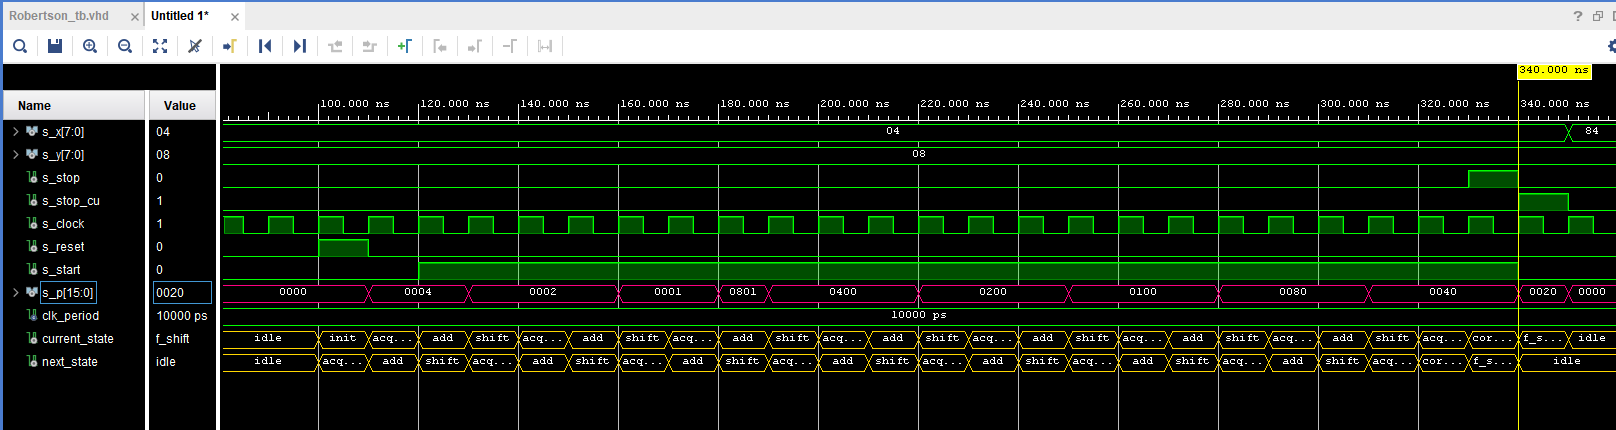
\includegraphics[width=16cm]{immagini/esercizio11/robertson_sim_xpos_ypos.png}
    \caption{Simulazione: X e Y positivi}
    \label{fig:robertson_sim_positivi}
\end{figure}

\begin{figure}[H]
    \centering
    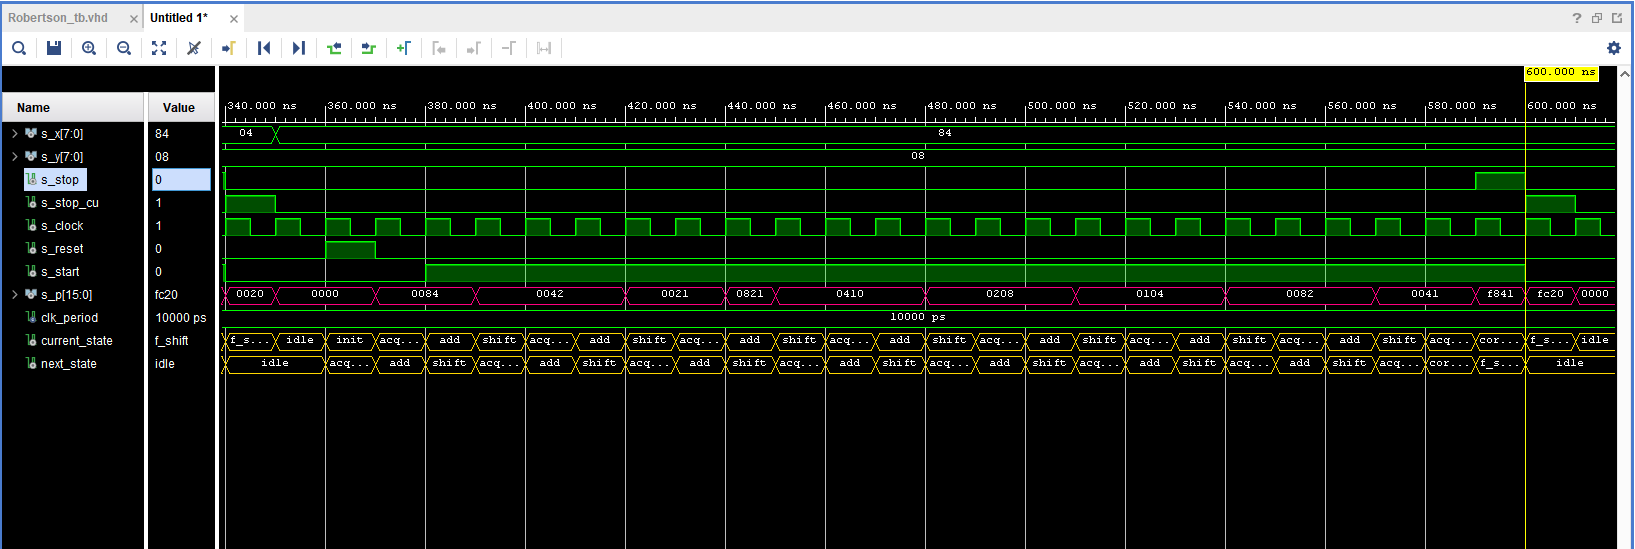
\includegraphics[width=16cm]{immagini/esercizio11/robertson_sim_xneg_ypos.png}
    \caption{Simulazione: X negativo e Y positivo}
    \label{fig:robertson_sim_xneg_ypos}
\end{figure}

\begin{figure}[H]
    \centering
    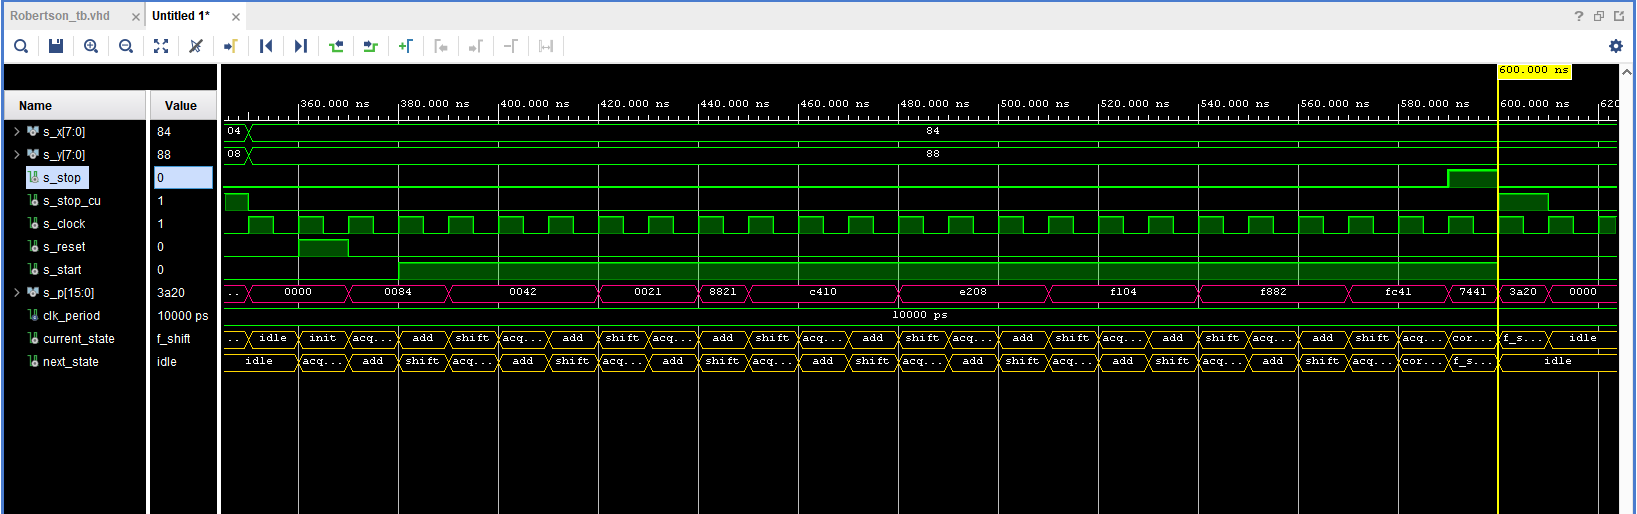
\includegraphics[width=16cm]{immagini/esercizio11/robertson_sim_xneg_yneg.png}
    \caption{Simulazione: X e Y negativi}
    \label{fig:robertson_sim_xneg_yneg}
\end{figure}


\begin{lstlisting} [language=VHDL, label=robertson_tb, caption=Testbench moltiplicatore di Robertson]
library IEEE;
use IEEE.STD_LOGIC_1164.ALL;
use IEEE.numeric_std;

entity Robertson_tb is
    --  Port ( );
end Robertson_tb;

architecture Behavioral of Robertson_tb is

    component  Robertson is
        port( clock, reset, start: in std_logic;
             X, Y: in std_logic_vector(7 downto 0);
             stop: out std_logic;
             P: out std_logic_vector(15 downto 0);
             stop_cu: out std_logic);
    end component Robertson;

    signal s_x, s_y: std_logic_vector (7 downto 0):="00000000";
    signal s_stop, s_stop_cu, s_clock, s_reset,s_start: std_logic:='0' ;
    signal s_p: std_logic_vector (15 downto 0):="0000000000000000";
    constant clk_period: time := 10ns;

begin

    uut: Robertson port map(
            clock=>s_clock ,
            reset=> s_reset ,
            start=> s_start,
            X=> s_x,
            Y=> s_y,
            stop=> s_stop,
            P=> s_p,
            stop_cu=> s_stop_cu
        );

    clock: process
    begin
        loop
            s_clock <= not s_clock;
            wait for clk_period/2;
        end loop;
    end process clock;

    process
    begin
    
    s_x<="00000100";
    s_y<="00001000";
    
    wait for 100ns;
    s_reset <= '1';
    wait for clk_period;
    s_reset <= '0';
    wait for clk_period;
    s_start <='1';

    wait until s_stop_cu='1';
    s_start <='0';
    
    wait for 10ns;

    s_x<="10000100";
    s_y<="00001000";
    
    wait for 10ns;
    s_reset <= '1';
    wait for clk_period ;
    s_reset <= '0';
    wait for clk_period ;
    s_start <='1';

    wait until s_stop_cu='1';
    s_start <='0';
  
   
    wait for 10ns;

    s_x<="10000100";
    s_y<="10001000";
    
    wait for 10ns;
    s_reset <= '1';
    wait for clk_period ;
    s_reset <= '0';
    wait for clk_period ;
    s_start <='1';

    wait until s_stop_cu='1';
    s_start <='0';
  
    wait;

    end process;

end Behavioral;

\end{lstlisting}
